\section{Bahnsteuerung}

\textbf{Trajektorie}: Bewegungen eines Roboters werden aufgefasst als Zustandsänderungen über die Zeit, die Einschränkungen berücksichtigen.

\textbf{Problem der Bahnsteuerung}:
\begin{itemize}
	\item Gegeben: Zustand $S_\text{Start}$ zum Startzeitpunkt und Zustand $S_\text{Ziel}$ zum Zielzeitpunkt
	\item Gesucht: Zwischenzustände $S_i$, damit Trajektorie stetig wird
\end{itemize}

\textbf{Darstellung der Zustände}: Zustände können dargestellt werden im
\begin{itemize}
	\item Konfigurationsraum: $\R^n$
	\item Arbeitsraum: $\R^3, \text{SE}(3)$
	\item Bahnsteuerung im Konfigurationsraum ist näher an der Ansteuerung der Teilsysteme des Roboter
	\item Bahnsteuerung im Arbeitsraum ist näher an der zu lösenden Aufgabe, zur Steuerung ist das Lösen der inversen Kinematik nötig
\end{itemize}

\begin{center}
	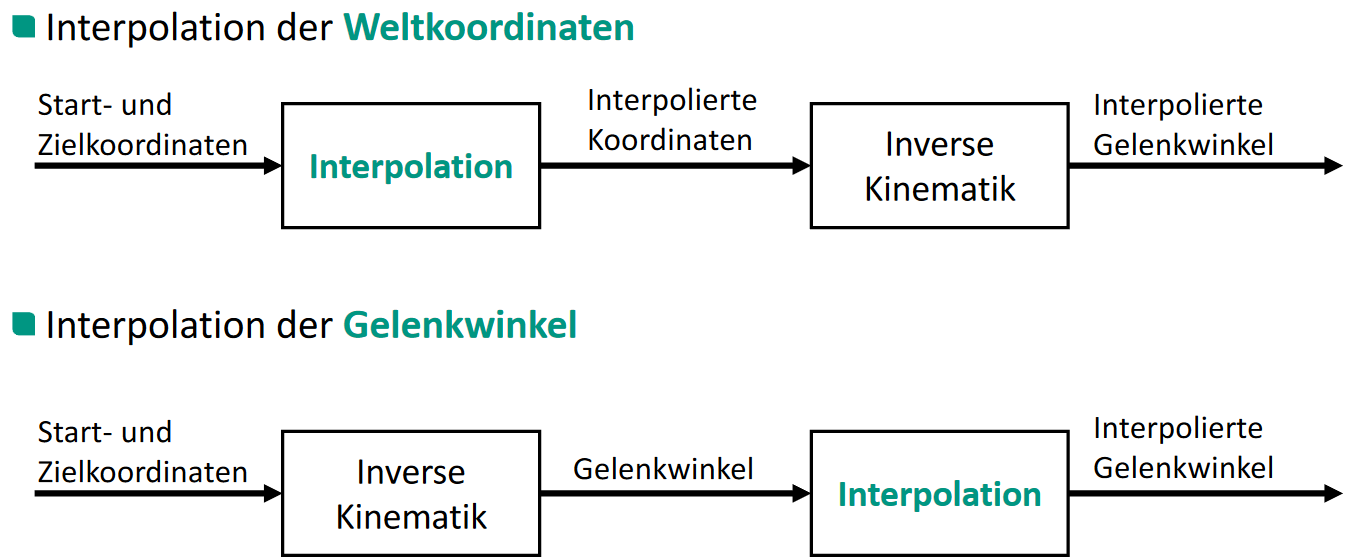
\includegraphics[width=0.7\textwidth]{images/interpolation.png}
\end{center}

\textbf{Bahnsteuerung im Konfigurationsraum}:
\begin{itemize}
	\item Bahnsteuerung als Funktion der Gelenkwinkelzustände
	\item Verlauf der punktweise in Gelenkwinkeln spezifizierten Bahn muss im Arbeitsraum nicht definiert sein
	\item Abfahren dieser punktweise spezifizierten Trajektorien \textbf{synchron} oder \textbf{asynchron}
\end{itemize}

\textbf{Bahnsteuerung im Arbeitsraum}:
\begin{itemize}
	\item Angabe der Trajektorie erfolgt als Funktion der Zustände des Roboters, z.B. Position, Geschwindigkeit, Beschleunigung
	\item \textbf{Continuous Path}: Endeffektor folgt in Position und Orientierung einer definierten Bahn
\end{itemize}

\textbf{Vor- und Nachteile der Darstellungen}:
\begin{itemize}
	\item \textbf{Arbeitsraum}:
	\begin{itemize}
		\item \textbf{Vorteile}: Bahn einfacher zu formulieren, Interpolation ist einfacher
		\item \textbf{Nachteile}: Inverse Kinematik für jeden Punkt der Trajektorie zu lösen, Geplante Trajektorie nicht immer ausführbar
	\end{itemize}
	\item \textbf{Konfigurationsraum}:
	\begin{itemize}
		\item \textbf{Vorteile}: Ansteuerung der Gelenke einfacher und Trajektorie ist eindeutig und berücksichtigt Gelenkwinkelgrenzen
		\item \textbf{Nachteile}: Interpolation für mehrere Gelenke, Formulierung der Trajektorie umständlicher
	\end{itemize}
\end{itemize}
\bigskip
\textbf{Punkt-zu-Punkt-Steuerung} (der Gelenkwinkel):
\begin{itemize}
	\item Roboter führt Punkt-zu-Punkt-Bewegung aus
	\item \textbf{Vorteile}: Berechnung der Gelenkwinkeltrajektorie ist einfach, Keine Probleme mit Singularitäten
	\item Sequenz von Gelenkwinkelvektoren: $\mathbf{q}(t_j)=(q_1(t_j),q_2(t_j),\ldots, q_n(t_j))^\top$ mit $q_i(t_j)$ ist Winkel von Gelenk $i$ zum Zeitpunkt $t_j$
	\item \textbf{Randbedingungen}:
	\begin{itemize}
		\item Start- und Zielzustand sind bekannt: $\mathbf{q}(t_0)=\mathbf{q}_\text{Start},\; \mathbf{q}(t_e)=\mathbf{q}_\text{Ziel}$
		\item Geschwindigkeiten zu Beginn und am Ende: $\mathbf{\dot{q}}(t_0)=x, \; \mathbf{\dot{q}}(t_e)=y$
		\item Gelenkwinkelbereich sowie Geschwindigkeiten und Beschleunigungen sind begrenzt: $\mathbf{q}_\text{min} < \mathbf{q}(t_j)<\mathbf{q}_\text{max},\; |\mathbf{\dot{q}}(t_j)|<\mathbf{\dot{q}}_\text{max},\; |\mathbf{\ddot{q}}(t_j)|<\mathbf{\ddot{q}}_\text{max}$
	\end{itemize}
	\item Interpolation für PTP mit \textbf{Rampenprofil}:
	\begin{itemize}
		\item \textbf{Vorteil}: Einfache Art zur Berechnung der Bahnparameter $s(t)$
		\item \textbf{Nachteil}: Sprungförmige Aufschaltung der Beschleunigung kann zu Eigenschwingungen von mechanischen Teilen führen
		\begin{center}
			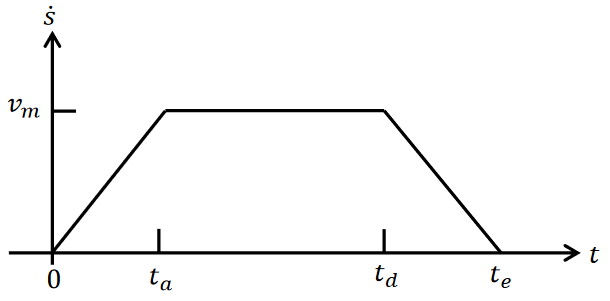
\includegraphics[width=0.4\textwidth]{images/rampenprofil.png}
		\end{center}
		\item \textbf{Berechnung der Parameter}: \textit{6/25-28}
	\end{itemize}
	\item Interpolation für PTP mit \textbf{Sinoidenprofil}:
	\begin{itemize}
		\item \textbf{Vorteil}: Roboter wird weniger beansprucht
		\item \textbf{Nachteil}: Längere Beschleunigungs- und Bremsphase als beim Rampenprofil
		\begin{center}
			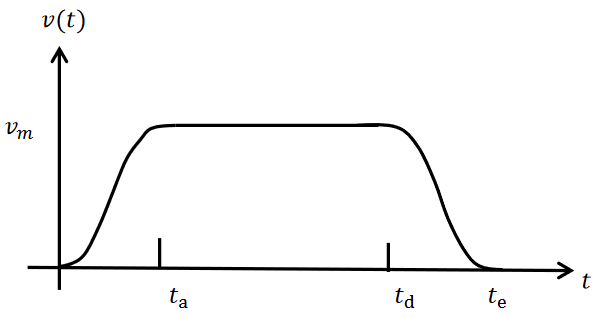
\includegraphics[width=0.4\textwidth]{images/sinoiden.png}
		\end{center}
		\item \textbf{Berechnung der Parameter}: \textit{6/31-32}
	\end{itemize}
	\begin{center}
		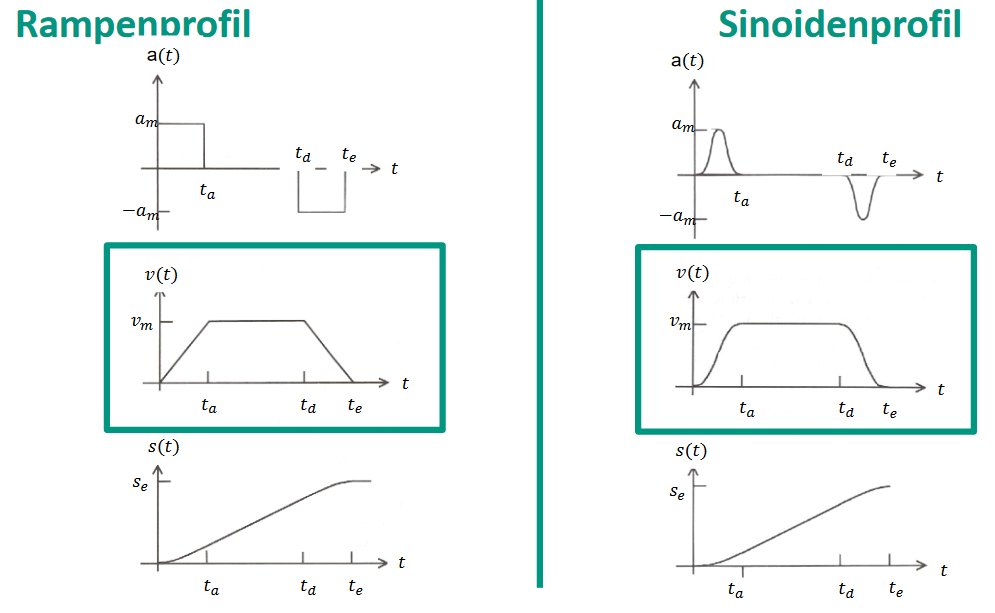
\includegraphics[width=0.7\textwidth]{images/rs.png}
	\end{center}
	\item \textbf{Asynchrone} und \textbf{synchrone} PTP-Bahnen:
	\begin{center}
		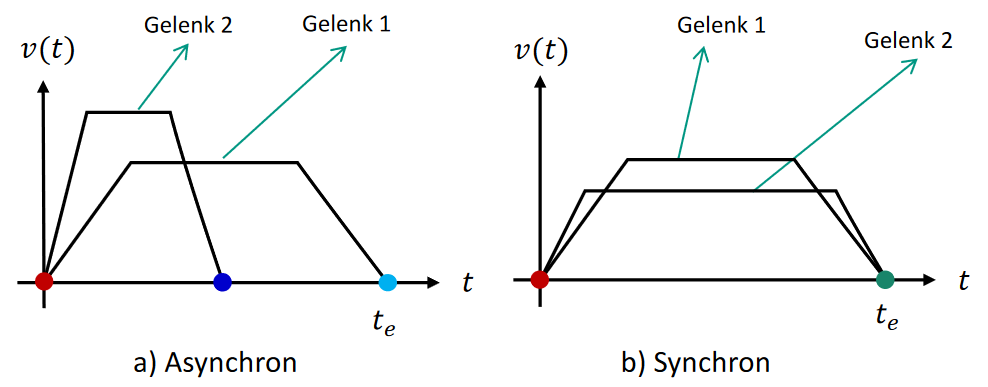
\includegraphics[width=0.6\textwidth]{images/asy-syn.png}
	\end{center}
	\begin{itemize}
		\item Asynchron: Jedes Gelenk wird sofort mit der maximalen Beschleunigung angesteuert. Jede Gelenkbewegung endet unabhängig von den anderen
		\item Synchron: Alle Gelenke beginnen und beenden ihre Bewegungen zum gleichen
		Zeitpunkt
	\end{itemize}
\end{itemize}
\bigskip
\textbf{Synchrone PTP-Bahnen}:
\begin{itemize}
	\item Setze die maximale Fahrzeit als Fahrzeit für alle Gelenke:
	$t_{e,i}=t_e=\max(t_{e,i})$
	\item Bei \textbf{vollsynchron}: Zusätzlich Beschleunigungszeit $t_a$ und Bremszeit $t_d$ bei allen Gelenken gleich
	\item Herleitung Formeln: \textit{5/38}
\end{itemize}
\bigskip
\textbf{Steuerung im Arbeitsraum}:
\begin{itemize}
	\item \textbf{Continuous Path}: Endeffektor folgt in Position und Orientierung einer definierten Bahn
	\item Pose des Endeffektors im Arbeitsraum gegeben durch Punkt $\mathbf{p}=(x,y,z)^\top\in\R^3$ und Orientierung $\boldsymbol{\omega}=(\alpha,\beta,\gamma)^\top\in\R^3$
	\begin{center}
		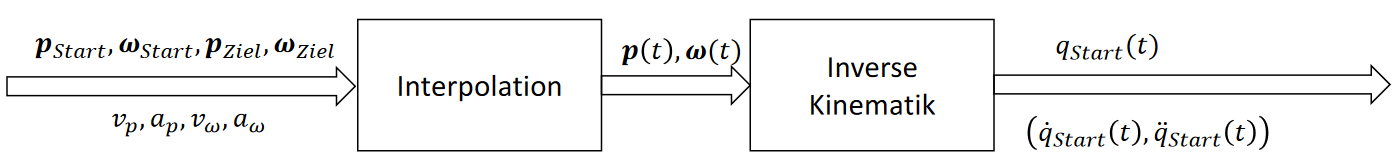
\includegraphics[width=\textwidth]{images/arbeitsraum.png}
	\end{center}
\end{itemize}
\bigskip
\textbf{Linearinterpolation}:
\begin{center}
	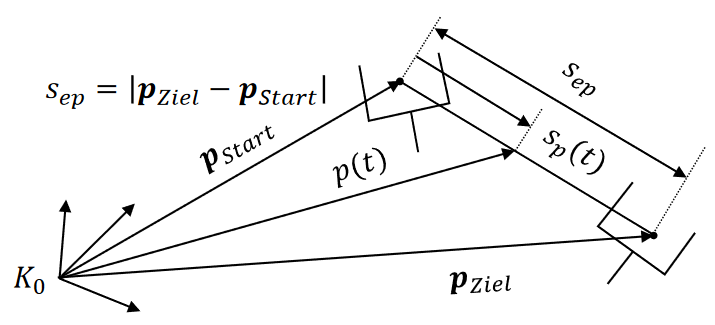
\includegraphics[width=0.4\textwidth]{images/lin.png}
\end{center}
\begin{itemize}
	\item $p(t)=\mathbf{p}_\text{Start}+\frac{s_p(t)}{s_{ep}}\cdot (\mathbf{p}_\text{Ziel}-\mathbf{p}_\text{Start})$
	\item \textbf{Berechnung} von $s_p(t)$ und $s_\omega(t)$: s. \textit{5/41-42}
\end{itemize}
\bigskip
\textbf{Segmentweise Bahninterpolation mit kubischen Splines}:
\begin{center}
	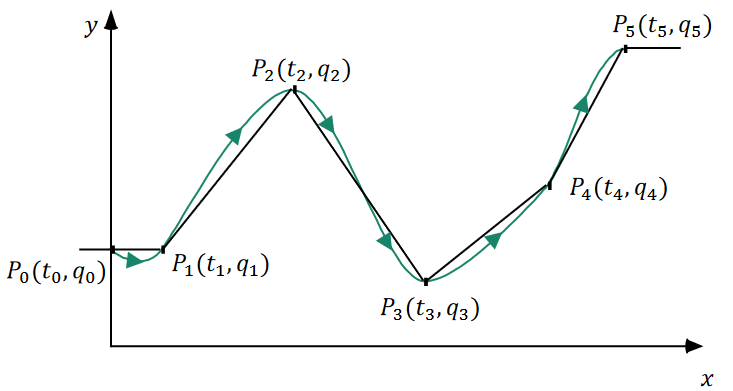
\includegraphics[width=0.5\textwidth]{images/splines.png}
\end{center}
\begin{itemize}
	\item Polynom $f(t)=a_0+a_1 t+a_2t^2+a_3t^3$
	\item \textbf{Gegeben}: Anfangspunkt $f(0)=s_a$, Endpunkt $f(t_e)=s_e$, Anfangsgeschwindigkeit $\dot{f}(0)=v_a$, Endgeschwindigkeit $\dot{f}(t_e)=v_e$
	\item \textbf{Gesucht}: Parameter $a_0,a_1,a_2,a_3\in\R$
	\item Berechnung s. \textit{5/46-50}
\end{itemize}
\bigskip
\textbf{Approximierte Bahnsteuerung}:
\begin{itemize}
	\item \textbf{Bahninterpolation}: Ausgeführte Bahn verläuft durch alle Stützpunkte der Trajektorie
	\item \textbf{Bahnapproximation}: Kontrollpunkte beeinflussen den Bahnverlauf und werden approximiert
	\begin{center}
		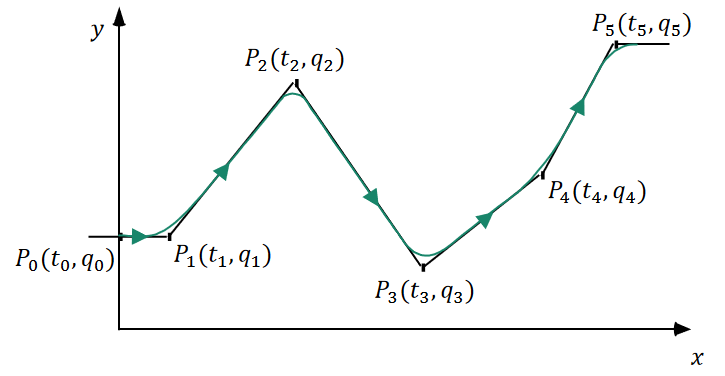
\includegraphics[width=0.5\textwidth]{images/approx.png}
	\end{center}
	\item \textbf{Überschleifen} vermeiden \enquote{roboterhafte} Bewegungen
\end{itemize}
\bigskip
\textbf{Approximation mit Bernsteinpolynomen}:
\begin{itemize}
	\item \textbf{Bézierkurven}: Im Unterschied zu kubischen Splines verlaufen Bézierkurven nicht durch alle Stützpunkte $\mathbf{P}_i$, sondern werden nur von ihnen beeinflusst
	$$P(t)=\sum\limits_{i=0}^{n} B_{i,n}(t)\mathbf{P}_i, \qquad \text{wobei } B_{i,n}(t)={n \choose i}t^i (1-t)^{n-i}$$
	das $i$-te \textbf{Bernsteinpolynom} vom Grad $n$ ist
	\item Annäherung an Bézierkurve durch \textbf{De-Casteljau-Algorithmus}, der darauf basiert, dass eine Bézierkurve geteilt und durch zwei aufeinanderfolgende Bézierkurven dargestellt wird
\end{itemize}
